
\documentclass[paper-main.tex]{subfiles}


\begin{document}
\han{add more text here from Changrong's ideas}

% wild speculation
We are currently working towards two future advancements for the optical microphone.


The first is to better isolate the experiment from the mains supply. 
The Raspberry Pi is USB powered and requires low power so it could be run off a commercial external phone battery. 
Everything else in the circuit, including the photodiode, is connected to the Pi, so this would isolate them electrically as well. 
The laser is DC powered through a converter, so should not introduce mains harmonics itself. 
Using the interferometer in a dark room and a sealed container could better isolate if from ambient light and air currents.
These changes may reduce or remove the $50\,{\rm Hz}$ harmonics from the data.
%With the interferometer in a dark room and under a box to better isolate from any ambient light or air currents, this would hopefully remove (or better separate) all sources of the 50Hz mains hum from the optical microphone.


The second advancement would be to achieve a full model of the transfer function of the system. 
Theoretically, if we had the correct transfer function, then signal recovery would only be limited by the signal-to-noise ratio as an optimal matched filter could be constructed.
The transfer function would need to start from the voltage sent to the speaker and end with the value recorded by the Pi, and include any non-linearities in the speaker audio production, the speaker-mirror coupling, the separation-intensity relation, and the photodiode reading. 
The sequence that the signal takes is shown in Figure~\ref{fig:pipeline_highlighted}.
In our investigation, we have currently only derived part of this sequence, the relation between a deflection of the mirror and the change in the intensity of the interference pattern at some point. 
We find this relation to be non-linear, see Appendix~\ref{app:intensity_derivation} for the derivation.


Asides from the transfer function, for extracting the speech there exists much literature~\cite{HMM_english} on using a hidden Markov model train to English phonemes to recognise speech.
Alternatively, machine learning solutions exist throughout the field that are able to compete~\cite{SEGAN} with statistical techniques like the logMMSE estimator.

To remove the mains hum we could also monitor it separately from the interferometer and subtract the sinusoids with the right phase and amplitude in real (not frequency) space to avoid the problems of Section~\ref{sec:simple_filters}. 
This could be done with the existing signals if the recording duration is long enough to precisely measure the phase and amplitude over a large number of cycles.


\begin{figure}
	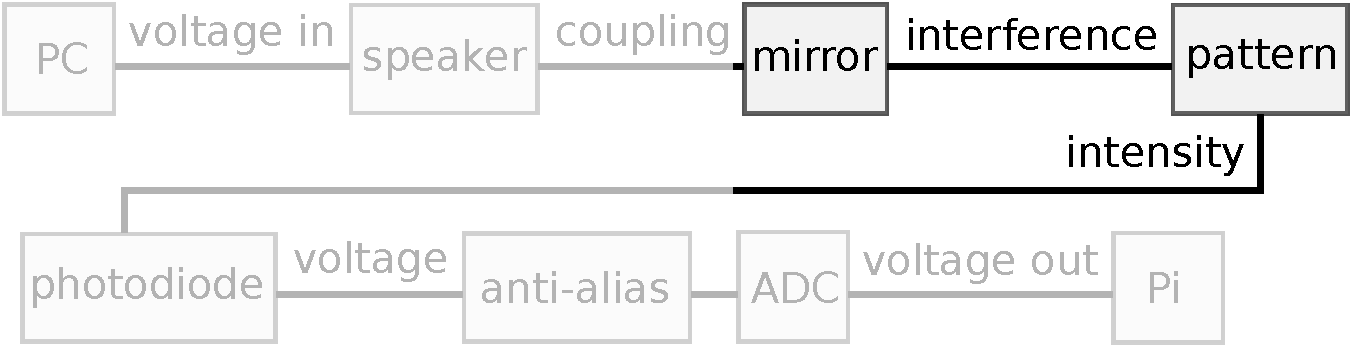
\includegraphics[width=.49\textwidth]{figures/pipeline_highlighted.pdf}
	\caption{Sequence of relations for optical microphone transfer function. The currently derived relation is highlighted.}
	\label{fig:pipeline_highlighted}
\end{figure}

\end{document}
